\documentclass{amsart} 
\usepackage{graphicx}
\graphicspath{{./}}
\usepackage[fontsize=14pt]{scrextend}
\usepackage{hyperref}
\usepackage{csvsimple}
\usepackage{epigraph}
\title{Right is Not Alone in the Universe}
\author{Zulfikar Moinuddin Ahmed}
\date{\today}
\begin{document}
\maketitle
\section{Motivation}
For most of my life I was left but I have since found more precise values that straddle left and right.  I realised that I should really do something for the right too since you are all my people and not just the left.  So today I will present the good news that you are not alone in the universe if you are right and everywhere on Earth there is right, across all ethnicities and languages.  Now now, I am not going to take up the right banner soon exactly, but I am more neutral now.

\section{Data from 68 countries}

Thanks to the World Values survey I examined the percent leaning right in sixty eight countries.  Here is the distribution of percent right.

\begin{verbatim}
> summary(fit.Right)
Asymmetric Generalized Hyperbolic Distribution:

Parameters:
    lambda    alpha.bar      mu
 -2.1495080  0.4024894  32.2949826 
 
    sigma      gamma 
11.0989092  4.0825377 

Call:
fit.ghypuv(data = polright$Right)

Optimization information:
log-Likelihood:                -258.7619 
AIC:                           527.5239
\end{verbatim}

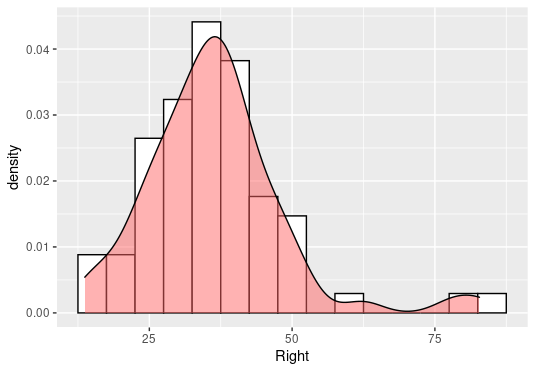
\includegraphics[scale=0.7]{right.png}

\section{Great work of Barndorff-Nielsen}

The Generalized Hyperbolic Distribution is the canonical distribution and is the outcome of a lifetime of fantastic work by Ole Barndorff-Nielsen and his colleagues and students.  The effort shows its true power here and in general in these Human Nature distributions across many countries because in all these besides the $(\mu,\sigma)$ of the Gaussian three additional parameters $(\lambda,\bar{\alpha},\gamma)$ are charged.  In other words, the GHD are not optional but necessary for science of Human Nature.  This is a general phenomenon, and one day it will be quite clear that without these highly intricate non-Gaussian precise distributions, science in this area would be quite sterile.  It is one of the most amazing features of Nature that Right leaning percentages with $N=68$ follows such a parametric distribution with such a good fit.  It is a great triumph for Levy process theory; it is a great triumph for the sophisticated work of Ole Barndorff-Nielsen and his colleague, and it is a great triumph for those seeking a Science of Human Nature by direct examination of global data rather than futile and unpleasant racial strife that sometimes infects some of these issues.  


\section{Data}

% latex table generated in R 3.6.3 by xtable 1.8-4 package
% Sun Apr  4 05:04:38 2021
\begin{table}[ht]
\centering
\begin{tabular}{rlr}
  \hline
 & Country & Right \\ 
  \hline
1 & Albania & 34.50 \\ 
  2 & Andorra & 25.10 \\ 
  3 & Azerbaijan & 42.10 \\ 
  4 & Argentina & 39.90 \\ 
  5 & Australia & 31.60 \\ 
  6 & Austria & 34.80 \\ 
  7 & Bangladesh & 82.80 \\ 
  8 & Armenia & 26.90 \\ 
  9 & Bolivia & 31.40 \\ 
  10 & Bosnia Herzegovina & 31.10 \\ 
  11 & Brazil & 22.60 \\ 
  12 & Bulgaria & 37.40 \\ 
  13 & Belarus & 19.10 \\ 
  14 & Chile & 23.50 \\ 
  15 & Taiwan ROC & 13.70 \\ 
  16 & Colombia & 46.80 \\ 
  17 & Croatia & 27.20 \\ 
  18 & Cyprus & 30.40 \\ 
  19 & Czech Rep. & 36.50 \\ 
  20 & Denmark & 38.20 \\ 
  21 & Ecuador & 37.20 \\ 
  22 & Ethiopia & 27.60 \\ 
  23 & Estonia & 30.30 \\ 
  24 & Finland & 49.40 \\ 
  25 & France & 29.70 \\ 
  26 & Georgia & 41.70 \\ 
  27 & Germany & 25.90 \\ 
  28 & Greece & 32.20 \\ 
  29 & Guatemala & 45.70 \\ 
  30 & Hong Kong SAR & 36.10 \\ 
  31 & Hungary & 41.50 \\ 
  32 & Iceland & 39.90 \\ 
  33 & Indonesia & 48.20 \\ 
  34 & Italy & 38.10 \\ 
  35 & Japan & 34.60 \\ 
  36 & South Korea & 43.80 \\ 
  37 & Lithuania & 34.40 \\ 
  38 & Macau SAR & 22.00 \\ 
  39 & Malaysia & 48.30 \\ 
  40 & Mexico & 40.60 \\ 
  41 & Montenegro & 14.80 \\ 
  42 & Netherlands & 45.50 \\ 
  43 & New Zealand & 36.60 \\ 
  44 & Nicaragua & 31.20 \\ 
  45 & Nigeria & 52.10 \\ 
  46 & Norway & 41.70 \\ 
  47 & Peru & 41.60 \\ 
  48 & Philippines & 62.30 \\ 
  49 & Poland & 39.00 \\ 
  50 & Portugal & 21.00 \\ 
  51 & Puerto Rico & 37.10 \\ 
  52 & Romania & 29.60 \\ 
  53 & Russia & 33.60 \\ 
  54 & Serbia & 26.50 \\ 
  55 & Slovakia & 36.00 \\ 
  56 & Slovenia & 16.60 \\ 
  57 & Zimbabwe & 36.70 \\ 
  58 & Spain & 26.80 \\ 
  59 & Sweden & 46.60 \\ 
  60 & Switzerland & 38.20 \\ 
  61 & Tajikistan & 78.10 \\ 
  62 & Thailand & 36.10 \\ 
  63 & Tunisia & 42.60 \\ 
  64 & Turkey & 52.00 \\ 
  65 & Ukraine & 24.10 \\ 
  66 & North Macedonia & 32.50 \\ 
  67 & United Kingdom & 32.80 \\ 
  68 & United States & 39.10 \\ 
   \hline
\end{tabular}
\end{table}

\end{document}
 


